\section{Vorüberlegungen}

\subsection{Datenquellen}
Ein Kernpunkt für die Entwicklung der Ingestion-Schnittstelle ist die Analyse der möglichen Datenquellen.
Da das System alle möglichen Datenquellen unterstützen soll, werden hier mögliche Typen dargestellt, mit denen sich alle Datenquellen abdecken lassen.
Dazu werden Merkmale betrachtet die Art und der Typ Ingestion bestimmen.
Mit der Art wird hier bezeichnet, ob die verwendeten Daten strukturiert, semi- oder unstrukturiert sind.
Da in der Vorarbeit, dem Masterprojekt, \textit{Apache Spark} verwendet wurde, ist dieser Punkt bereits abgedeckt und fällt bei der Entwicklung nicht weiter ins Gewicht.

Als zweites gibt es die Typen, die hier beschreiben, wie Daten in das System gelangen.
Dazu gibt es zwei Merkmale, in denen sich die Ingestions unterscheiden können.
Das erste ist, ob die Unterscheidung zwischen Push- und Pull-Prinzip.
Bei dem Push-Prinzip werden die zu speichernden Daten mit der Anfrage an das System gesendet und bei dem Pull-Prinzip muss dass System die Daten aus einer Quelle laden.
Die zweite Unterscheidung findet statt in einmalige in kontinuierliche Ingestion.
Diese Unterscheidungen können, müssen aber nicht, von der Datenquelle abhängig sein.
Als Beispiel gibt es Datenströme, die laufend Daten senden und somit eine Ingestion benötigen, die auch laufend Daten annimmt.
Im Gegensatz dazu gibt es Datenbanken, bei denen das System die Daten aus der Quelle laden muss und somit die Ingestion sowohl einmalig als auch kontinuierlich sein kann.

Aus diesen Unterscheidungen ergeben sich die vier mögliche Verarbeitungswege, die in \ref{fig:ingestion_types} zu sehen sind.
Sowohl für Push- und Pull-Prinzip kann eine einfache Ingestion ausgeführt werden, die sich für kontinuierliche Pull-Ingestions wiederholt.
Bei einer kontinuierlichen Ingestion, bei der Daten an das System gesendet werden, handelt es sich um Datenströme, die eine extra Verarbeitung erfordern.

\begin{figure}
    \centering
    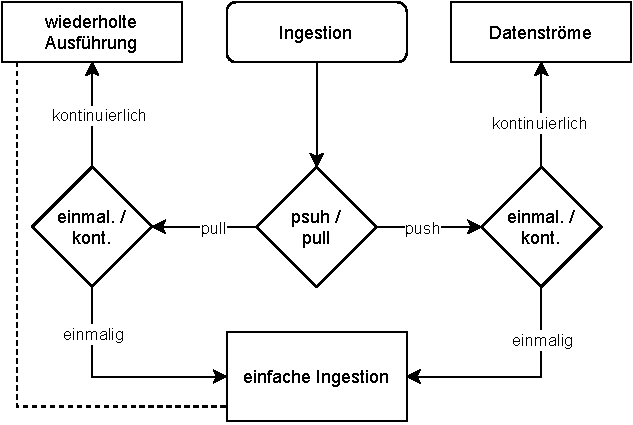
\includegraphics{Grafiken/ingestion-types.pdf}
    \caption{Ingestion-Typen}
    \label{fig:ingestion_types}
\end{figure}

\subsection{Architektur Ansatz}
Die Anwendung, die im Masterprojekt entwickelt wurde ist eine monolithische Anwendung.
Das bedeutet, dass die gesamte Software als ein großes Programm entwickelt und bereitgestellt wird.
Solche Anwendungen sind zwar in der Entwicklung und Bereitstellung leicht umzusetzen, haben aber größere Nachteile in Bereichen wie Fehlertoleranz und Wartung.
Im Vergleich dazu gibt es die Microservice-Architektur, bei der mehrere kleine Anwendungen entwickelt werden, die bestimmte aufgaben übernehmen und am gesamt Problem gemeinsam beteiligt sind.
Diese haben im, wie von \textcite{microservices} dargestellt, mehrere Vorteile gegenüber monolithischen Anwendungen.
Die Wartung fällt bei vielen kleinen Programmen leichter, da sie übersichtlicher und verständlicher sind als ein großes und Fehler betreffen jeweils nur den Microservice selbst.
Außerdem ist es einfacher bestimmte Aspekte der Software zu skalieren und bei Updates bleibt eine höhere Verfügbarkeit, da nur ein kleiner Teil des Systems neu gestartet werden muss.

Als Nachteil wird aber auch erwähnt, dass die Bereitstellung einer Mircoservice-Architektur komplexer ist als die einer monolithischen.
Diese Problem kann aber mit Container-Lösung wie \textit{Docker}\footnote{https://www.docker.com/} vereinfacht werden.
Dabei werden sogenannte Contianer aus den Mircoservices gebaut, die ähnlich zu einer virtuellen Maschine sind und einen bestimmten Zustand speichern.
Beim Starten eines Containers wird genau in diesem Zustand eingestiegen, so dass man ohne großen Aufwand zum Beispiel einen Webserver mit einer bestimmt Anwendung auf verschiedenen System starten kann, ohne sich um deren Installationen kümmern zu müssen.

Auf Grund der genannten Vorteile soll das Data Lake System und damit die Ingestion als Microservice-Architektur entwickelt werden.
Das bedeutet, dass Punkte gefunden werden müssen, an denen sich das System gut in einzelene Anwendungen trennen lässt.